\documentclass[12pt]{article}
\usepackage{minted}
\usepackage{graphicx}
\usepackage[margin=0.25in]{geometry}

\begin{document} 
	\noindent
	Dan Jandel C. De Ramos\\
	BSCpE 2-1\\
	Made with \LaTeX \\
	\\
	Activity 1\\
	Source Code:
	
	\begin{minted}[tabsize=5]{java}         
/*
* Written by: Dan Jandel C. De Ramos
* Polytechnic University of the Philippines Biñan
* Bachelor of Science in Computer Engineering 2-1
*/

public class Activity_1{
	public static void main(String[]args){         
		
		//The data stored here are for the sake of examples only and are not 100% accurate        
		String name_1 = "Dan Jandel C. De Ramos";        
		char gender = 'M';
		char pesoSign = '\u20B1';
		boolean maritalStatus = false;
		byte numberOfChildren = 0;
		short birthYear = 2003;
		int salary = 65536;  
		long netAsset = 89414685416L;
		double weight = 69.42;
		float gpa = 1.88f;
		
		System.out.println();
		
		System.out.println(" \u2022 Activity # 1 \u2022 \n");
		System.out.println("Name: " + name_1);
		System.out.println("Gender: " + gender);
		System.out.println("Married: " + maritalStatus);
		System.out.println("Number of Children: " + numberOfChildren);
		System.out.println("Year of birth: " + birthYear);
		System.out.println("Salary: " + pesoSign + " " + salary);
		System.out.println("Net Asset: " + pesoSign + " " + netAsset);
		System.out.println("Weight: " + weight + "kg");
		System.out.println("GPA: " + gpa);       
		
		System.out.println();        
	}
}
	\end{minted}
\clearpage
\noindent
Output:\\
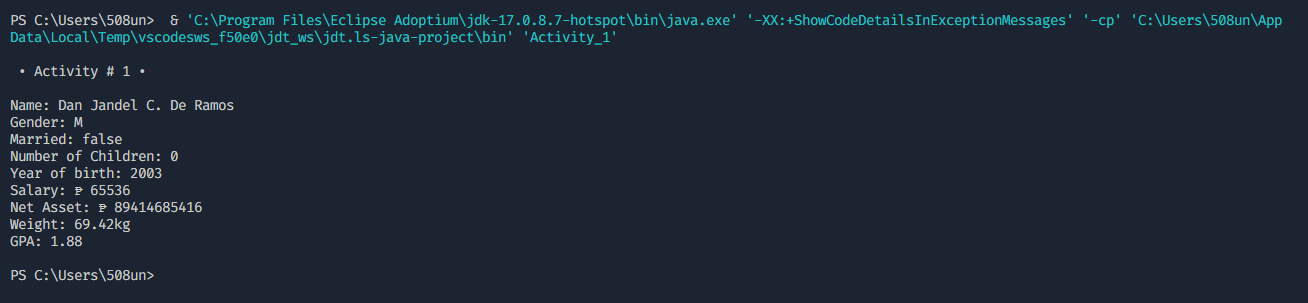
\includegraphics[width=\textwidth]{output}
\end{document}